\documentclass[a4paper]{book}
\usepackage{a4wide}
\usepackage{makeidx}
\usepackage{fancyhdr}
\usepackage{graphicx}
\usepackage{multicol}
\usepackage{float}
\usepackage{textcomp}
\usepackage{alltt}
\usepackage{times}
\usepackage{ifpdf}
\ifpdf
\usepackage[pdftex,
            pagebackref=true,
            colorlinks=true,
            linkcolor=blue,
            unicode
           ]{hyperref}
\else
\usepackage[ps2pdf,
            pagebackref=true,
            colorlinks=true,
            linkcolor=blue,
            unicode
           ]{hyperref}
\usepackage{pspicture}
\fi
\usepackage[utf8]{inputenc}
\usepackage{doxygen}
\makeindex
\setcounter{tocdepth}{3}
\renewcommand{\footrulewidth}{0.4pt}
\begin{document}
\begin{titlepage}
\vspace*{7cm}
\begin{center}
{\Large Domogik }\\
\vspace*{1cm}
{\large Generated by Doxygen 1.5.6}\\
\vspace*{0.5cm}
{\small Wed Feb 4 13:54:18 2009}\\
\end{center}
\end{titlepage}
\clearemptydoublepage
\pagenumbering{roman}
\tableofcontents
\clearemptydoublepage
\pagenumbering{arabic}
\chapter{Directory Hierarchy}
\section{Directories}
This directory hierarchy is sorted roughly, but not completely, alphabetically:\begin{CompactList}
\item \contentsline{section}{config}{\pageref{dir_cee9c79587f570ceb8ce290779602f9e}}{}
\item \contentsline{section}{control}{\pageref{dir_ab51fe5183395bffca5b27dcaf8dba7d}}{}
\item \contentsline{section}{xpl}{\pageref{dir_bcacd883f70269073ed4fd6ad0018512}}{}
\end{CompactList}

\chapter{Class Index}
\section{Class Hierarchy}
This inheritance list is sorted roughly, but not completely, alphabetically:\begin{CompactList}
\item \contentsline{section}{domogik::xpl::trigger::Condition}{\pageref{classdomogik_1_1xpl_1_1trigger_1_1Condition}}{}
\begin{CompactList}
\item \contentsline{section}{domogik::xpl::trigger::AND}{\pageref{classdomogik_1_1xpl_1_1trigger_1_1AND}}{}
\item \contentsline{section}{domogik::xpl::trigger::NOT}{\pageref{classdomogik_1_1xpl_1_1trigger_1_1NOT}}{}
\item \contentsline{section}{domogik::xpl::trigger::OR}{\pageref{classdomogik_1_1xpl_1_1trigger_1_1OR}}{}
\item \contentsline{section}{domogik::xpl::trigger::stateCond}{\pageref{classdomogik_1_1xpl_1_1trigger_1_1stateCond}}{}
\item \contentsline{section}{domogik::xpl::trigger::timeCond}{\pageref{classdomogik_1_1xpl_1_1trigger_1_1timeCond}}{}
\end{CompactList}
\item \contentsline{section}{generate\_\-config::ConfigManager}{\pageref{classgenerate__config_1_1ConfigManager}}{}
\item \contentsline{section}{domogik::control::models::DeviceCategory}{\pageref{classdomogik_1_1control_1_1models_1_1DeviceCategory}}{}
\item \contentsline{section}{domogik::doxypy::FSM}{\pageref{classdomogik_1_1doxypy_1_1FSM}}{}
\item \contentsline{section}{generate\_\-config::genericPluginConfig}{\pageref{classgenerate__config_1_1genericPluginConfig}}{}
\begin{CompactList}
\item \contentsline{section}{generate\_\-config::datetimeConfig}{\pageref{classgenerate__config_1_1datetimeConfig}}{}
\item \contentsline{section}{generate\_\-config::generalConfig}{\pageref{classgenerate__config_1_1generalConfig}}{}
\item \contentsline{section}{generate\_\-config::senderConfig}{\pageref{classgenerate__config_1_1senderConfig}}{}
\item \contentsline{section}{generate\_\-config::triggerConfig}{\pageref{classgenerate__config_1_1triggerConfig}}{}
\item \contentsline{section}{generate\_\-config::x10Config}{\pageref{classgenerate__config_1_1x10Config}}{}
\end{CompactList}
\item \contentsline{section}{domogik::xpl::xPLAPI::Listener}{\pageref{classdomogik_1_1xpl_1_1xPLAPI_1_1Listener}}{}
\item \contentsline{section}{domogik::xpl::trigger::ListenerBuilder}{\pageref{classdomogik_1_1xpl_1_1trigger_1_1ListenerBuilder}}{}
\item \contentsline{section}{domogik::common::configloader::Loader}{\pageref{classdomogik_1_1common_1_1configloader_1_1Loader}}{}
\item \contentsline{section}{domogik::common::logger::Logger}{\pageref{classdomogik_1_1common_1_1logger_1_1Logger}}{}
\item \contentsline{section}{domogik::xpl::xPLAPI::Manager}{\pageref{classdomogik_1_1xpl_1_1xPLAPI_1_1Manager}}{}
\item \contentsline{section}{domogik::xpl::xPLAPI::Message}{\pageref{classdomogik_1_1xpl_1_1xPLAPI_1_1Message}}{}
\item \contentsline{section}{domogik::xpl::onewire::OneWire}{\pageref{classdomogik_1_1xpl_1_1onewire_1_1OneWire}}{}
\item \contentsline{section}{domogik::xpl::onewire::OneWireException}{\pageref{classdomogik_1_1xpl_1_1onewire_1_1OneWireException}}{}
\item \contentsline{section}{domogik::control::SampleDataHelper::SampleDataHelper}{\pageref{classdomogik_1_1control_1_1SampleDataHelper_1_1SampleDataHelper}}{}
\item \contentsline{section}{domogik::xpl::x10API::X10API}{\pageref{classdomogik_1_1xpl_1_1x10API_1_1X10API}}{}
\item \contentsline{section}{domogik::xpl::x10API::X10Exception}{\pageref{classdomogik_1_1xpl_1_1x10API_1_1X10Exception}}{}
\item \contentsline{section}{domogik::xpl::datetime::xPLDateTime}{\pageref{classdomogik_1_1xpl_1_1datetime_1_1xPLDateTime}}{}
\item \contentsline{section}{domogik::xpl::xPLAPI::XPLException}{\pageref{classdomogik_1_1xpl_1_1xPLAPI_1_1XPLException}}{}
\item \contentsline{section}{domogik::control::XPLHelper::XPLHelper}{\pageref{classdomogik_1_1control_1_1XPLHelper_1_1XPLHelper}}{}
\item \contentsline{section}{domogik::xpl::xPLAPI::xPLTimer}{\pageref{classdomogik_1_1xpl_1_1xPLAPI_1_1xPLTimer}}{}
\end{CompactList}

\chapter{Class Index}
\section{Class List}
Here are the classes, structs, unions and interfaces with brief descriptions:\begin{CompactList}
\item\contentsline{section}{\hyperlink{classdomogik_1_1xpl_1_1trigger_1_1AND}{domogik::xpl::trigger::AND} (Implementation for the \hyperlink{classdomogik_1_1xpl_1_1trigger_1_1AND}{AND} operator )}{\pageref{classdomogik_1_1xpl_1_1trigger_1_1AND}}{}
\item\contentsline{section}{\hyperlink{classdomogik_1_1xpl_1_1trigger_1_1Condition}{domogik::xpl::trigger::Condition} (Parent class for each condition A condition can be a node : it store 1 or 2 other conditions, or a final node : it just implements some eval of the condition )}{\pageref{classdomogik_1_1xpl_1_1trigger_1_1Condition}}{}
\item\contentsline{section}{\hyperlink{classgenerate__config_1_1ConfigManager}{generate\_\-config::ConfigManager} (General config manager which can ask user about config settings, check results and write config file )}{\pageref{classgenerate__config_1_1ConfigManager}}{}
\item\contentsline{section}{\hyperlink{classgenerate__config_1_1datetimeConfig}{generate\_\-config::datetimeConfig} (Ask the user for specific config for the xPL datetime module )}{\pageref{classgenerate__config_1_1datetimeConfig}}{}
\item\contentsline{section}{\hyperlink{classdomogik_1_1control_1_1models_1_1DeviceCategory}{domogik::control::models::DeviceCategory} (Examples : temperature, heating, lighting, music, )}{\pageref{classdomogik_1_1control_1_1models_1_1DeviceCategory}}{}
\item\contentsline{section}{\hyperlink{classdomogik_1_1doxypy_1_1FSM}{domogik::doxypy::FSM} (Implements a finite state machine )}{\pageref{classdomogik_1_1doxypy_1_1FSM}}{}
\item\contentsline{section}{\hyperlink{classgenerate__config_1_1generalConfig}{generate\_\-config::generalConfig} (Ask the user for general configuration and write results )}{\pageref{classgenerate__config_1_1generalConfig}}{}
\item\contentsline{section}{\hyperlink{classgenerate__config_1_1genericPluginConfig}{generate\_\-config::genericPluginConfig} (Generic list for plugins )}{\pageref{classgenerate__config_1_1genericPluginConfig}}{}
\item\contentsline{section}{\hyperlink{classdomogik_1_1xpl_1_1xPLAPI_1_1Listener}{domogik::xpl::xPLAPI::Listener} (\hyperlink{classdomogik_1_1xpl_1_1xPLAPI_1_1Listener}{Listener} are objects which are able to check if a message match some filter and to call a function if they do )}{\pageref{classdomogik_1_1xpl_1_1xPLAPI_1_1Listener}}{}
\item\contentsline{section}{\hyperlink{classdomogik_1_1xpl_1_1trigger_1_1ListenerBuilder}{domogik::xpl::trigger::ListenerBuilder} (Class to parse an expression and create appropriated listener )}{\pageref{classdomogik_1_1xpl_1_1trigger_1_1ListenerBuilder}}{}
\item\contentsline{section}{\hyperlink{classdomogik_1_1common_1_1configloader_1_1Loader}{domogik::common::configloader::Loader} (Parse Domogik config files )}{\pageref{classdomogik_1_1common_1_1configloader_1_1Loader}}{}
\item\contentsline{section}{\hyperlink{classdomogik_1_1common_1_1logger_1_1Logger}{domogik::common::logger::Logger} (\hyperlink{classdomogik_1_1common_1_1logger_1_1Logger}{Logger} for the xPL system )}{\pageref{classdomogik_1_1common_1_1logger_1_1Logger}}{}
\item\contentsline{section}{\hyperlink{classdomogik_1_1xpl_1_1xPLAPI_1_1Manager}{domogik::xpl::xPLAPI::Manager} (\hyperlink{classdomogik_1_1xpl_1_1xPLAPI_1_1Manager}{Manager} is the main component of the system You can run many managers on different port Each manager will send an heartbeat message on broadcast on port 3865 to announce itself to the xPL Hub )}{\pageref{classdomogik_1_1xpl_1_1xPLAPI_1_1Manager}}{}
\item\contentsline{section}{\hyperlink{classdomogik_1_1xpl_1_1xPLAPI_1_1Message}{domogik::xpl::xPLAPI::Message} (\hyperlink{classdomogik_1_1xpl_1_1xPLAPI_1_1Message}{Message} is the object for all data received form the network )}{\pageref{classdomogik_1_1xpl_1_1xPLAPI_1_1Message}}{}
\item\contentsline{section}{\hyperlink{classdomogik_1_1xpl_1_1trigger_1_1NOT}{domogik::xpl::trigger::NOT} (Implementation for the \hyperlink{classdomogik_1_1xpl_1_1trigger_1_1NOT}{NOT} operator )}{\pageref{classdomogik_1_1xpl_1_1trigger_1_1NOT}}{}
\item\contentsline{section}{\hyperlink{classdomogik_1_1xpl_1_1onewire_1_1OneWire}{domogik::xpl::onewire::OneWire} (Manage \hyperlink{classdomogik_1_1xpl_1_1onewire_1_1OneWire}{OneWire} )}{\pageref{classdomogik_1_1xpl_1_1onewire_1_1OneWire}}{}
\item\contentsline{section}{\hyperlink{classdomogik_1_1xpl_1_1onewire_1_1OneWireException}{domogik::xpl::onewire::OneWireException} (\hyperlink{classdomogik_1_1xpl_1_1onewire_1_1OneWire}{OneWire} exception )}{\pageref{classdomogik_1_1xpl_1_1onewire_1_1OneWireException}}{}
\item\contentsline{section}{\hyperlink{classdomogik_1_1xpl_1_1trigger_1_1OR}{domogik::xpl::trigger::OR} (Implementation for the \hyperlink{classdomogik_1_1xpl_1_1trigger_1_1OR}{OR} operator )}{\pageref{classdomogik_1_1xpl_1_1trigger_1_1OR}}{}
\item\contentsline{section}{\hyperlink{classdomogik_1_1control_1_1SampleDataHelper_1_1SampleDataHelper}{domogik::control::SampleDataHelper::SampleDataHelper} (Class to load / clear sample data )}{\pageref{classdomogik_1_1control_1_1SampleDataHelper_1_1SampleDataHelper}}{}
\item\contentsline{section}{\hyperlink{classgenerate__config_1_1senderConfig}{generate\_\-config::senderConfig} (Ask the user for specific config for the xPL sender )}{\pageref{classgenerate__config_1_1senderConfig}}{}
\item\contentsline{section}{\hyperlink{classdomogik_1_1xpl_1_1trigger_1_1stateCond}{domogik::xpl::trigger::stateCond} (Implementation of the state condition This allows user to describe a condition on any item of the system )}{\pageref{classdomogik_1_1xpl_1_1trigger_1_1stateCond}}{}
\item\contentsline{section}{\hyperlink{classdomogik_1_1xpl_1_1trigger_1_1timeCond}{domogik::xpl::trigger::timeCond} (Implementation of the time condition This allows user to describe time periods like cron )}{\pageref{classdomogik_1_1xpl_1_1trigger_1_1timeCond}}{}
\item\contentsline{section}{\hyperlink{classgenerate__config_1_1triggerConfig}{generate\_\-config::triggerConfig} (Ask the user for specific config for the xPL sender )}{\pageref{classgenerate__config_1_1triggerConfig}}{}
\item\contentsline{section}{\hyperlink{classdomogik_1_1xpl_1_1x10API_1_1X10API}{domogik::xpl::x10API::X10API} (This class define some facilities to use X10 )}{\pageref{classdomogik_1_1xpl_1_1x10API_1_1X10API}}{}
\item\contentsline{section}{\hyperlink{classgenerate__config_1_1x10Config}{generate\_\-config::x10Config} (Ask the user for specific config for X10 xPL module )}{\pageref{classgenerate__config_1_1x10Config}}{}
\item\contentsline{section}{\hyperlink{classdomogik_1_1xpl_1_1x10API_1_1X10Exception}{domogik::xpl::x10API::X10Exception} (X10 exception )}{\pageref{classdomogik_1_1xpl_1_1x10API_1_1X10Exception}}{}
\item\contentsline{section}{\hyperlink{classdomogik_1_1xpl_1_1datetime_1_1xPLDateTime}{domogik::xpl::datetime::xPLDateTime} (Send date and time on the xPL network every minute )}{\pageref{classdomogik_1_1xpl_1_1datetime_1_1xPLDateTime}}{}
\item\contentsline{section}{\hyperlink{classdomogik_1_1xpl_1_1xPLAPI_1_1XPLException}{domogik::xpl::xPLAPI::XPLException} (XPL exception )}{\pageref{classdomogik_1_1xpl_1_1xPLAPI_1_1XPLException}}{}
\item\contentsline{section}{\hyperlink{classdomogik_1_1control_1_1XPLHelper_1_1XPLHelper}{domogik::control::XPLHelper::XPLHelper} (Utility class for xPL )}{\pageref{classdomogik_1_1control_1_1XPLHelper_1_1XPLHelper}}{}
\item\contentsline{section}{\hyperlink{classdomogik_1_1xpl_1_1xPLAPI_1_1xPLTimer}{domogik::xpl::xPLAPI::xPLTimer} (XPLTimer will call a callback function each n seconds )}{\pageref{classdomogik_1_1xpl_1_1xPLAPI_1_1xPLTimer}}{}
\end{CompactList}

\chapter{Directory Documentation}
\hypertarget{dir_cee9c79587f570ceb8ce290779602f9e}{
\section{config/ Directory Reference}
\label{dir_cee9c79587f570ceb8ce290779602f9e}\index{config/ Directory Reference@{config/ Directory Reference}}
}
\subsection*{Files}
\begin{CompactItemize}
\item 
file \textbf{generate\_\-config.py}
\end{CompactItemize}

\hypertarget{dir_ab51fe5183395bffca5b27dcaf8dba7d}{
\section{control/ Directory Reference}
\label{dir_ab51fe5183395bffca5b27dcaf8dba7d}\index{control/ Directory Reference@{control/ Directory Reference}}
}
\subsection*{Files}
\begin{CompactItemize}
\item 
file \textbf{\_\-\_\-init\_\-\_\-.py}
\item 
file \textbf{admin.py}
\item 
file \textbf{forms.py}
\item 
file \textbf{models.py}
\item 
file \textbf{SampleDataHelper.py}
\item 
file \textbf{urls.py}
\item 
file \textbf{views.py}
\end{CompactItemize}

\hypertarget{dir_bcacd883f70269073ed4fd6ad0018512}{
\section{xpl/ Directory Reference}
\label{dir_bcacd883f70269073ed4fd6ad0018512}\index{xpl/ Directory Reference@{xpl/ Directory Reference}}
}
\subsection*{Files}
\begin{CompactItemize}
\item 
file \textbf{\_\-\_\-init\_\-\_\-.py}
\item 
file \textbf{datetime.py}
\item 
file \textbf{dawndusk.py}
\item 
file \textbf{main\_\-DawnDusk.py}
\item 
file \textbf{onewire.py}
\item 
file \textbf{onewire\_\-main.py}
\item 
file \textbf{send.py}
\item 
file \textbf{trigger.py}
\item 
file \textbf{x10\_\-main.py}
\item 
file \textbf{x10API.py}
\item 
file \textbf{xPLAPI.py}
\end{CompactItemize}

\chapter{Class Documentation}
\hypertarget{classgenerate__config_1_1ConfigManager}{
\section{generate\_\-config::ConfigManager Class Reference}
\label{classgenerate__config_1_1ConfigManager}\index{generate\_\-config::ConfigManager@{generate\_\-config::ConfigManager}}
}
\subsection*{Public Member Functions}
\begin{CompactItemize}
\item 
def \hyperlink{classgenerate__config_1_1ConfigManager_9d306a6d2e086a1dd9175423ad415798}{\_\-\_\-init\_\-\_\-}
\item 
def \hyperlink{classgenerate__config_1_1ConfigManager_277e7238684d6750957bf2981e0eec14}{ask}
\item 
def \hyperlink{classgenerate__config_1_1ConfigManager_50916dd9f4420c45c85048c3448dfd9e}{write}
\end{CompactItemize}
\subsection*{Private Attributes}
\begin{CompactItemize}
\item 
\hypertarget{classgenerate__config_1_1ConfigManager_c7cc7bdff5ea3be7296ab6400ad0f61f}{
\textbf{\_\-settings}}
\label{classgenerate__config_1_1ConfigManager_c7cc7bdff5ea3be7296ab6400ad0f61f}

\item 
\hypertarget{classgenerate__config_1_1ConfigManager_4df37a3c3f5e0d781cf0344774e1eff0}{
\textbf{\_\-session}}
\label{classgenerate__config_1_1ConfigManager_4df37a3c3f5e0d781cf0344774e1eff0}

\end{CompactItemize}


\subsection{Detailed Description}


\footnotesize\begin{verbatim}
General config manager which can ask user about config settings, check results and write config file
\end{verbatim}
\normalsize
 

\subsection{Member Function Documentation}
\hypertarget{classgenerate__config_1_1ConfigManager_9d306a6d2e086a1dd9175423ad415798}{
\index{generate\_\-config::ConfigManager@{generate\_\-config::ConfigManager}!\_\-\_\-init\_\-\_\-@{\_\-\_\-init\_\-\_\-}}
\index{\_\-\_\-init\_\-\_\-@{\_\-\_\-init\_\-\_\-}!generate_config::ConfigManager@{generate\_\-config::ConfigManager}}
\subsubsection[\_\-\_\-init\_\-\_\-]{\setlength{\rightskip}{0pt plus 5cm}def generate\_\-config::ConfigManager::\_\-\_\-init\_\-\_\- ( {\em self}, \/   {\em settings} = {\tt \mbox{[}\mbox{]}}, \/   {\em session} = {\tt None})}}
\label{classgenerate__config_1_1ConfigManager_9d306a6d2e086a1dd9175423ad415798}




\footnotesize\begin{verbatim}
Constructor 
@param settings List of tuples defining parameters to ask user for : {'name','question','check_regex',['proposed_val1','proposed_val2']}
check_regex can be None
Proposed value list can be None. If it isn't, the first value is taken as default choice
\end{verbatim}
\normalsize
 \hypertarget{classgenerate__config_1_1ConfigManager_277e7238684d6750957bf2981e0eec14}{
\index{generate\_\-config::ConfigManager@{generate\_\-config::ConfigManager}!ask@{ask}}
\index{ask@{ask}!generate_config::ConfigManager@{generate\_\-config::ConfigManager}}
\subsubsection[ask]{\setlength{\rightskip}{0pt plus 5cm}def generate\_\-config::ConfigManager::ask ( {\em self})}}
\label{classgenerate__config_1_1ConfigManager_277e7238684d6750957bf2981e0eec14}




\footnotesize\begin{verbatim}
Ask the user for each entry of self._settings
\end{verbatim}
\normalsize
 \hypertarget{classgenerate__config_1_1ConfigManager_50916dd9f4420c45c85048c3448dfd9e}{
\index{generate\_\-config::ConfigManager@{generate\_\-config::ConfigManager}!write@{write}}
\index{write@{write}!generate_config::ConfigManager@{generate\_\-config::ConfigManager}}
\subsubsection[write]{\setlength{\rightskip}{0pt plus 5cm}def generate\_\-config::ConfigManager::write ( {\em self}, \/   {\em filename}, \/   {\em datas}, \/   {\em section} = {\tt None})}}
\label{classgenerate__config_1_1ConfigManager_50916dd9f4420c45c85048c3448dfd9e}




\footnotesize\begin{verbatim}
Write data in a filename. May define a section
\end{verbatim}
\normalsize
 

The documentation for this class was generated from the following file:\begin{CompactItemize}
\item 
config/generate\_\-config.py\end{CompactItemize}

\hypertarget{classgenerate__config_1_1datetimeConfig}{
\section{generate\_\-config::datetimeConfig Class Reference}
\label{classgenerate__config_1_1datetimeConfig}\index{generate\_\-config::datetimeConfig@{generate\_\-config::datetimeConfig}}
}
Inheritance diagram for generate\_\-config::datetimeConfig::\begin{figure}[H]
\begin{center}
\leavevmode
\includegraphics[height=2cm]{classgenerate__config_1_1datetimeConfig}
\end{center}
\end{figure}
\subsection*{Public Member Functions}
\begin{CompactItemize}
\item 
\hypertarget{classgenerate__config_1_1datetimeConfig_84bd0d1f10cb05b3513a3da208cab7bb}{
def \textbf{\_\-\_\-init\_\-\_\-}}
\label{classgenerate__config_1_1datetimeConfig_84bd0d1f10cb05b3513a3da208cab7bb}

\end{CompactItemize}


\subsection{Detailed Description}


\footnotesize\begin{verbatim}
Ask the user for specific config for the xPL datetime module
\end{verbatim}
\normalsize
 

The documentation for this class was generated from the following file:\begin{CompactItemize}
\item 
config/generate\_\-config.py\end{CompactItemize}

\hypertarget{classgenerate__config_1_1generalConfig}{
\section{generate\_\-config::generalConfig Class Reference}
\label{classgenerate__config_1_1generalConfig}\index{generate\_\-config::generalConfig@{generate\_\-config::generalConfig}}
}
\subsection*{Public Member Functions}
\begin{CompactItemize}
\item 
def \hyperlink{classgenerate__config_1_1generalConfig_470de1124f102c64ad61af244dbac061}{\_\-\_\-init\_\-\_\-}
\end{CompactItemize}


\subsection{Detailed Description}


\footnotesize\begin{verbatim}
Ask the user for general configuration and write results
\end{verbatim}
\normalsize
 

\subsection{Member Function Documentation}
\hypertarget{classgenerate__config_1_1generalConfig_470de1124f102c64ad61af244dbac061}{
\index{generate\_\-config::generalConfig@{generate\_\-config::generalConfig}!\_\-\_\-init\_\-\_\-@{\_\-\_\-init\_\-\_\-}}
\index{\_\-\_\-init\_\-\_\-@{\_\-\_\-init\_\-\_\-}!generate_config::generalConfig@{generate\_\-config::generalConfig}}
\subsubsection[\_\-\_\-init\_\-\_\-]{\setlength{\rightskip}{0pt plus 5cm}def generate\_\-config::generalConfig::\_\-\_\-init\_\-\_\- ( {\em self})}}
\label{classgenerate__config_1_1generalConfig_470de1124f102c64ad61af244dbac061}




\footnotesize\begin{verbatim}
Ask user for general parameters of Domogik to create the main config file
\end{verbatim}
\normalsize
 

The documentation for this class was generated from the following file:\begin{CompactItemize}
\item 
config/generate\_\-config.py\end{CompactItemize}

\hypertarget{classgenerate__config_1_1genericPluginConfig}{
\section{generate\_\-config::genericPluginConfig Class Reference}
\label{classgenerate__config_1_1genericPluginConfig}\index{generate\_\-config::genericPluginConfig@{generate\_\-config::genericPluginConfig}}
}
Generic list for plugins.  


Inheritance diagram for generate\_\-config::genericPluginConfig::\begin{figure}[H]
\begin{center}
\leavevmode
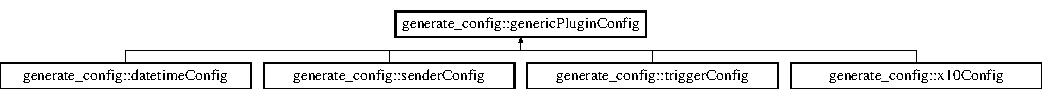
\includegraphics[height=0.961373cm]{classgenerate__config_1_1genericPluginConfig}
\end{center}
\end{figure}
\subsection*{Public Member Functions}
\begin{CompactItemize}
\item 
\hypertarget{classgenerate__config_1_1genericPluginConfig_6e5142c1890303123b37a9b1015601c8}{
def \textbf{\_\-\_\-init\_\-\_\-}}
\label{classgenerate__config_1_1genericPluginConfig_6e5142c1890303123b37a9b1015601c8}

\item 
\hypertarget{classgenerate__config_1_1genericPluginConfig_5e6843b1a07f91051930ac9ae93f4494}{
def \textbf{askandwrite}}
\label{classgenerate__config_1_1genericPluginConfig_5e6843b1a07f91051930ac9ae93f4494}

\item 
\hypertarget{classgenerate__config_1_1genericPluginConfig_aae7b874b8371f63fb170cb9f3682b12}{
def \textbf{getvalue}}
\label{classgenerate__config_1_1genericPluginConfig_aae7b874b8371f63fb170cb9f3682b12}

\end{CompactItemize}
\subsection*{Public Attributes}
\begin{CompactItemize}
\item 
\hypertarget{classgenerate__config_1_1genericPluginConfig_4d6143782994ef3d177b90f38f4512c4}{
\textbf{informations}}
\label{classgenerate__config_1_1genericPluginConfig_4d6143782994ef3d177b90f38f4512c4}

\item 
\hypertarget{classgenerate__config_1_1genericPluginConfig_e8a1d20ad1774f98d48f58f908a62216}{
\textbf{result}}
\label{classgenerate__config_1_1genericPluginConfig_e8a1d20ad1774f98d48f58f908a62216}

\end{CompactItemize}


\subsection{Detailed Description}
Generic list for plugins. 

The documentation for this class was generated from the following file:\begin{CompactItemize}
\item 
config/generate\_\-config.py\end{CompactItemize}

\hypertarget{classxPLAPI_1_1Listener}{
\section{xPLAPI::Listener Class Reference}
\label{classxPLAPI_1_1Listener}\index{xPLAPI::Listener@{xPLAPI::Listener}}
}
\subsection*{Public Member Functions}
\begin{CompactItemize}
\item 
def \hyperlink{classxPLAPI_1_1Listener_31c68a5ad76d56eff1b78dd646a18e58}{\_\-\_\-init\_\-\_\-}
\item 
\hypertarget{classxPLAPI_1_1Listener_f61ad8e3de5cfd5c8d69aee1cbddaedd}{
def \textbf{getFilter}}
\label{classxPLAPI_1_1Listener_f61ad8e3de5cfd5c8d69aee1cbddaedd}

\item 
\hypertarget{classxPLAPI_1_1Listener_0b3088bf2df0f408d0f2c15989386cca}{
def \textbf{getCb}}
\label{classxPLAPI_1_1Listener_0b3088bf2df0f408d0f2c15989386cca}

\item 
def \hyperlink{classxPLAPI_1_1Listener_a6e3c6a481054d9ff921507b784b0f12}{new\_\-message}
\item 
def \hyperlink{classxPLAPI_1_1Listener_ff3b74767e27828d084af4d34e3fd20e}{add\_\-filter}
\item 
def \hyperlink{classxPLAPI_1_1Listener_babc7a4d6a30876fda2fc593942069b0}{del\_\-filter}
\item 
def \hyperlink{classxPLAPI_1_1Listener_e719472458dd324763b91364a3991df1}{get\_\-filter\_\-list}
\end{CompactItemize}
\subsection*{Private Attributes}
\begin{CompactItemize}
\item 
\hypertarget{classxPLAPI_1_1Listener_64bd36ca836cbd2d56417dc17b83f8cf}{
\textbf{\_\-callback}}
\label{classxPLAPI_1_1Listener_64bd36ca836cbd2d56417dc17b83f8cf}

\item 
\hypertarget{classxPLAPI_1_1Listener_daa53232362ca9b704223184d9ef612f}{
\textbf{\_\-filter}}
\label{classxPLAPI_1_1Listener_daa53232362ca9b704223184d9ef612f}

\end{CompactItemize}


\subsection{Detailed Description}


\footnotesize\begin{verbatim}
Listener are objects which are able to check if a message
match some filter and to call a function if they do
\end{verbatim}
\normalsize
 

\subsection{Member Function Documentation}
\hypertarget{classxPLAPI_1_1Listener_31c68a5ad76d56eff1b78dd646a18e58}{
\index{xPLAPI::Listener@{xPLAPI::Listener}!\_\-\_\-init\_\-\_\-@{\_\-\_\-init\_\-\_\-}}
\index{\_\-\_\-init\_\-\_\-@{\_\-\_\-init\_\-\_\-}!xPLAPI::Listener@{xPLAPI::Listener}}
\subsubsection[\_\-\_\-init\_\-\_\-]{\setlength{\rightskip}{0pt plus 5cm}def xPLAPI::Listener::\_\-\_\-init\_\-\_\- ( {\em self}, \/   {\em cb}, \/   {\em manager}, \/   {\em filter} = {\tt \{\}})}}
\label{classxPLAPI_1_1Listener_31c68a5ad76d56eff1b78dd646a18e58}




\footnotesize\begin{verbatim}
The listener will get all messages from the manager and parse them.
If a message match the filter, then the callback function will be called
with the message as parameter
@param cb : the callback function
@param manager : the manager instance
@param filter : dictionnary { key : value } 
\end{verbatim}
\normalsize
 \hypertarget{classxPLAPI_1_1Listener_a6e3c6a481054d9ff921507b784b0f12}{
\index{xPLAPI::Listener@{xPLAPI::Listener}!new\_\-message@{new\_\-message}}
\index{new\_\-message@{new\_\-message}!xPLAPI::Listener@{xPLAPI::Listener}}
\subsubsection[new\_\-message]{\setlength{\rightskip}{0pt plus 5cm}def xPLAPI::Listener::new\_\-message ( {\em self}, \/   {\em message})}}
\label{classxPLAPI_1_1Listener_a6e3c6a481054d9ff921507b784b0f12}




\footnotesize\begin{verbatim}
This is the function which is called by the manager when a message arrives
The goal of this function is to check if message match filter rules, and to
call the callback function if it does
\end{verbatim}
\normalsize
 \hypertarget{classxPLAPI_1_1Listener_ff3b74767e27828d084af4d34e3fd20e}{
\index{xPLAPI::Listener@{xPLAPI::Listener}!add\_\-filter@{add\_\-filter}}
\index{add\_\-filter@{add\_\-filter}!xPLAPI::Listener@{xPLAPI::Listener}}
\subsubsection[add\_\-filter]{\setlength{\rightskip}{0pt plus 5cm}def xPLAPI::Listener::add\_\-filter ( {\em self}, \/   {\em key}, \/   {\em value})}}
\label{classxPLAPI_1_1Listener_ff3b74767e27828d084af4d34e3fd20e}




\footnotesize\begin{verbatim}
Add a filter rule. No distinction between conf and data
If the key already exists, the new value is used
\end{verbatim}
\normalsize
 \hypertarget{classxPLAPI_1_1Listener_babc7a4d6a30876fda2fc593942069b0}{
\index{xPLAPI::Listener@{xPLAPI::Listener}!del\_\-filter@{del\_\-filter}}
\index{del\_\-filter@{del\_\-filter}!xPLAPI::Listener@{xPLAPI::Listener}}
\subsubsection[del\_\-filter]{\setlength{\rightskip}{0pt plus 5cm}def xPLAPI::Listener::del\_\-filter ( {\em self}, \/   {\em key})}}
\label{classxPLAPI_1_1Listener_babc7a4d6a30876fda2fc593942069b0}




\footnotesize\begin{verbatim}
Remove a rule from filter list
If the key isn't in the list, do nothing
\end{verbatim}
\normalsize
 \hypertarget{classxPLAPI_1_1Listener_e719472458dd324763b91364a3991df1}{
\index{xPLAPI::Listener@{xPLAPI::Listener}!get\_\-filter\_\-list@{get\_\-filter\_\-list}}
\index{get\_\-filter\_\-list@{get\_\-filter\_\-list}!xPLAPI::Listener@{xPLAPI::Listener}}
\subsubsection[get\_\-filter\_\-list]{\setlength{\rightskip}{0pt plus 5cm}def xPLAPI::Listener::get\_\-filter\_\-list ( {\em self})}}
\label{classxPLAPI_1_1Listener_e719472458dd324763b91364a3991df1}




\footnotesize\begin{verbatim}
Get all the filter items
\end{verbatim}
\normalsize
 

The documentation for this class was generated from the following file:\begin{CompactItemize}
\item 
xpl/xPLAPI.py\end{CompactItemize}

\hypertarget{classconfigloader_1_1Loader}{
\section{configloader::Loader Class Reference}
\label{classconfigloader_1_1Loader}\index{configloader::Loader@{configloader::Loader}}
}
\subsection*{Public Member Functions}
\begin{CompactItemize}
\item 
def \hyperlink{classconfigloader_1_1Loader_f16abb85a49b17461dcc647f4a2d5e00}{\_\-\_\-init\_\-\_\-}
\item 
def \hyperlink{classconfigloader_1_1Loader_52f1433b0ea290e45661b7473c3a68d4}{load}
\end{CompactItemize}
\subsection*{Public Attributes}
\begin{CompactItemize}
\item 
\hypertarget{classconfigloader_1_1Loader_1a7a816df2d21c388cbb544c79caa065}{
\textbf{main\_\-conf\_\-name}}
\label{classconfigloader_1_1Loader_1a7a816df2d21c388cbb544c79caa065}

\item 
\hypertarget{classconfigloader_1_1Loader_44604dd7b77716499655a4f39453a13d}{
\textbf{module\_\-name}}
\label{classconfigloader_1_1Loader_44604dd7b77716499655a4f39453a13d}

\end{CompactItemize}


\subsection{Detailed Description}


\footnotesize\begin{verbatim}
Parse Domogik config files
\end{verbatim}
\normalsize
 

\subsection{Member Function Documentation}
\hypertarget{classconfigloader_1_1Loader_f16abb85a49b17461dcc647f4a2d5e00}{
\index{configloader::Loader@{configloader::Loader}!\_\-\_\-init\_\-\_\-@{\_\-\_\-init\_\-\_\-}}
\index{\_\-\_\-init\_\-\_\-@{\_\-\_\-init\_\-\_\-}!configloader::Loader@{configloader::Loader}}
\subsubsection[\_\-\_\-init\_\-\_\-]{\setlength{\rightskip}{0pt plus 5cm}def configloader::Loader::\_\-\_\-init\_\-\_\- ( {\em self}, \/   {\em module\_\-name} = {\tt None})}}
\label{classconfigloader_1_1Loader_f16abb85a49b17461dcc647f4a2d5e00}




\footnotesize\begin{verbatim}
Load the configuration for a part of the Domogik system
@param module_name name of the module to load config from
\end{verbatim}
\normalsize
 \hypertarget{classconfigloader_1_1Loader_52f1433b0ea290e45661b7473c3a68d4}{
\index{configloader::Loader@{configloader::Loader}!load@{load}}
\index{load@{load}!configloader::Loader@{configloader::Loader}}
\subsubsection[load]{\setlength{\rightskip}{0pt plus 5cm}def configloader::Loader::load ( {\em self})}}
\label{classconfigloader_1_1Loader_52f1433b0ea290e45661b7473c3a68d4}




\footnotesize\begin{verbatim}
Parse the config
@return pair (main_config, plugin_config)
\end{verbatim}
\normalsize
 

The documentation for this class was generated from the following file:\begin{CompactItemize}
\item 
xpl/configloader.py\end{CompactItemize}

\hypertarget{classxPLAPI_1_1Manager}{
\section{xPLAPI::Manager Class Reference}
\label{classxPLAPI_1_1Manager}\index{xPLAPI::Manager@{xPLAPI::Manager}}
}
\subsection*{Public Member Functions}
\begin{CompactItemize}
\item 
def \hyperlink{classxPLAPI_1_1Manager_57252f423d02495f598f858e9c699d38}{\_\-\_\-init\_\-\_\-}
\item 
def \hyperlink{classxPLAPI_1_1Manager_c955c61a27cc1b91885632576bf2c13d}{leave}
\item 
def \hyperlink{classxPLAPI_1_1Manager_98293b52fe5999a6bdfbe1cf17d08eb7}{send}
\item 
def \hyperlink{classxPLAPI_1_1Manager_e40b7a76258786cbf63ae2374b28c053}{add\_\-listener}
\end{CompactItemize}
\subsection*{Private Member Functions}
\begin{CompactItemize}
\item 
def \hyperlink{classxPLAPI_1_1Manager_c4032a0074505d88356fbc04468ca01c}{\_\-SendHeartbeat}
\item 
def \hyperlink{classxPLAPI_1_1Manager_f3b6bb58d65bbacf144099c29389481b}{\_\-run\_\-thread\_\-monitor}
\end{CompactItemize}
\subsection*{Private Attributes}
\begin{CompactItemize}
\item 
\hypertarget{classxPLAPI_1_1Manager_3ed8de348b50c251796cdca17dbd2aa3}{
\textbf{\_\-buff}}
\label{classxPLAPI_1_1Manager_3ed8de348b50c251796cdca17dbd2aa3}

\item 
\hypertarget{classxPLAPI_1_1Manager_2bc7b3100a53ad071f76f3b681c52661}{
\textbf{\_\-port}}
\label{classxPLAPI_1_1Manager_2bc7b3100a53ad071f76f3b681c52661}

\item 
\hypertarget{classxPLAPI_1_1Manager_c683222401e40e3d2fd218263a1450c0}{
\textbf{\_\-ip}}
\label{classxPLAPI_1_1Manager_c683222401e40e3d2fd218263a1450c0}

\item 
\hypertarget{classxPLAPI_1_1Manager_704810400121d4f606126b0a639e22c6}{
\textbf{\_\-source}}
\label{classxPLAPI_1_1Manager_704810400121d4f606126b0a639e22c6}

\item 
\hypertarget{classxPLAPI_1_1Manager_86ca9159e4cb44b28540f7afc82743e2}{
\textbf{\_\-listeners}}
\label{classxPLAPI_1_1Manager_86ca9159e4cb44b28540f7afc82743e2}

\item 
\hypertarget{classxPLAPI_1_1Manager_4c26907af60a5c4cb2e88b68a51273b7}{
\textbf{\_\-UDPSock}}
\label{classxPLAPI_1_1Manager_4c26907af60a5c4cb2e88b68a51273b7}

\item 
\hypertarget{classxPLAPI_1_1Manager_290fb2f20ababa2c8a5d5f897372b815}{
\textbf{\_\-h\_\-timer}}
\label{classxPLAPI_1_1Manager_290fb2f20ababa2c8a5d5f897372b815}

\item 
\hypertarget{classxPLAPI_1_1Manager_d6ccff08bbaa94d7ce89ce1bd847708c}{
\textbf{\_\-stop\_\-thread}}
\label{classxPLAPI_1_1Manager_d6ccff08bbaa94d7ce89ce1bd847708c}

\item 
\hypertarget{classxPLAPI_1_1Manager_b1941f7867b7a151b21fd865f7ac9f82}{
\textbf{\_\-network}}
\label{classxPLAPI_1_1Manager_b1941f7867b7a151b21fd865f7ac9f82}

\end{CompactItemize}


\subsection{Detailed Description}


\footnotesize\begin{verbatim}
Manager is the main component of the system
You can run many managers on different port
Each manager will send an heartbeat message on broadcast on port 3865
to announce itself to the xPL Hub
\end{verbatim}
\normalsize
 

\subsection{Member Function Documentation}
\hypertarget{classxPLAPI_1_1Manager_57252f423d02495f598f858e9c699d38}{
\index{xPLAPI::Manager@{xPLAPI::Manager}!\_\-\_\-init\_\-\_\-@{\_\-\_\-init\_\-\_\-}}
\index{\_\-\_\-init\_\-\_\-@{\_\-\_\-init\_\-\_\-}!xPLAPI::Manager@{xPLAPI::Manager}}
\subsubsection[\_\-\_\-init\_\-\_\-]{\setlength{\rightskip}{0pt plus 5cm}def xPLAPI::Manager::\_\-\_\-init\_\-\_\- ( {\em self}, \/   {\em ip} = {\tt \char`\"{}0.0.0.0\char`\"{}}, \/   {\em source} = {\tt \char`\"{}xpl-monitor.python\char`\"{}}, \/   {\em port} = {\tt 3865})}}
\label{classxPLAPI_1_1Manager_57252f423d02495f598f858e9c699d38}




\footnotesize\begin{verbatim}
Create a new manager instance
@param ip : IP to listen to (default 0.0.0.0)
@param source : source name of the application
@param port : port to listen to (default 3865)
\end{verbatim}
\normalsize
 \hypertarget{classxPLAPI_1_1Manager_c955c61a27cc1b91885632576bf2c13d}{
\index{xPLAPI::Manager@{xPLAPI::Manager}!leave@{leave}}
\index{leave@{leave}!xPLAPI::Manager@{xPLAPI::Manager}}
\subsubsection[leave]{\setlength{\rightskip}{0pt plus 5cm}def xPLAPI::Manager::leave ( {\em self})}}
\label{classxPLAPI_1_1Manager_c955c61a27cc1b91885632576bf2c13d}




\footnotesize\begin{verbatim}
Stop threads and leave the Manager
\end{verbatim}
\normalsize
 \hypertarget{classxPLAPI_1_1Manager_98293b52fe5999a6bdfbe1cf17d08eb7}{
\index{xPLAPI::Manager@{xPLAPI::Manager}!send@{send}}
\index{send@{send}!xPLAPI::Manager@{xPLAPI::Manager}}
\subsubsection[send]{\setlength{\rightskip}{0pt plus 5cm}def xPLAPI::Manager::send ( {\em self}, \/   {\em message})}}
\label{classxPLAPI_1_1Manager_98293b52fe5999a6bdfbe1cf17d08eb7}




\footnotesize\begin{verbatim}
This function allows you to send an xPL message on the Bus
Be carreful, there is no check on message correctness
\end{verbatim}
\normalsize
 \hypertarget{classxPLAPI_1_1Manager_c4032a0074505d88356fbc04468ca01c}{
\index{xPLAPI::Manager@{xPLAPI::Manager}!\_\-SendHeartbeat@{\_\-SendHeartbeat}}
\index{\_\-SendHeartbeat@{\_\-SendHeartbeat}!xPLAPI::Manager@{xPLAPI::Manager}}
\subsubsection[\_\-SendHeartbeat]{\setlength{\rightskip}{0pt plus 5cm}def xPLAPI::Manager::\_\-SendHeartbeat ( {\em self})\hspace{0.3cm}{\tt  \mbox{[}private\mbox{]}}}}
\label{classxPLAPI_1_1Manager_c4032a0074505d88356fbc04468ca01c}




\footnotesize\begin{verbatim}
Send heartbeat message in broadcast on the network, on the bus port (3865)
This make the application able to be discovered by the hub
\end{verbatim}
\normalsize
 \hypertarget{classxPLAPI_1_1Manager_f3b6bb58d65bbacf144099c29389481b}{
\index{xPLAPI::Manager@{xPLAPI::Manager}!\_\-run\_\-thread\_\-monitor@{\_\-run\_\-thread\_\-monitor}}
\index{\_\-run\_\-thread\_\-monitor@{\_\-run\_\-thread\_\-monitor}!xPLAPI::Manager@{xPLAPI::Manager}}
\subsubsection[\_\-run\_\-thread\_\-monitor]{\setlength{\rightskip}{0pt plus 5cm}def xPLAPI::Manager::\_\-run\_\-thread\_\-monitor ( {\em self})\hspace{0.3cm}{\tt  \mbox{[}private\mbox{]}}}}
\label{classxPLAPI_1_1Manager_f3b6bb58d65bbacf144099c29389481b}




\footnotesize\begin{verbatim}
The monitor thread receive all messages on the connection and check
them to see if the target is the application.
If it is, call all listeners
\end{verbatim}
\normalsize
 \hypertarget{classxPLAPI_1_1Manager_e40b7a76258786cbf63ae2374b28c053}{
\index{xPLAPI::Manager@{xPLAPI::Manager}!add\_\-listener@{add\_\-listener}}
\index{add\_\-listener@{add\_\-listener}!xPLAPI::Manager@{xPLAPI::Manager}}
\subsubsection[add\_\-listener]{\setlength{\rightskip}{0pt plus 5cm}def xPLAPI::Manager::add\_\-listener ( {\em self}, \/   {\em listener})}}
\label{classxPLAPI_1_1Manager_e40b7a76258786cbf63ae2374b28c053}




\footnotesize\begin{verbatim}
Add a listener on the list of the manager
@param listener : the listener instance
\end{verbatim}
\normalsize
 

The documentation for this class was generated from the following file:\begin{CompactItemize}
\item 
xpl/xPLAPI.py\end{CompactItemize}

\hypertarget{classxPLAPI_1_1Message}{
\section{xPLAPI::Message Class Reference}
\label{classxPLAPI_1_1Message}\index{xPLAPI::Message@{xPLAPI::Message}}
}
\subsection*{Public Member Functions}
\begin{CompactItemize}
\item 
def \hyperlink{classxPLAPI_1_1Message_f1efb1186af373f1ce3d107be47e3f3f}{\_\-\_\-init\_\-\_\-}
\item 
def \hyperlink{classxPLAPI_1_1Message_a24b962cfffbd90f1cb79a2c20e581e6}{set\_\-type}
\item 
def \hyperlink{classxPLAPI_1_1Message_55aad8c9b685e349f7e3d3f58b6ff5aa}{get\_\-type}
\item 
def \hyperlink{classxPLAPI_1_1Message_560b2b7685ee99a34ea7d01e7135477c}{set\_\-schema}
\item 
def \hyperlink{classxPLAPI_1_1Message_58df48b064cb3d59780a51c67136e88a}{get\_\-schema}
\item 
def \hyperlink{classxPLAPI_1_1Message_014808e1035dcea973692d4d823427ce}{set\_\-conf\_\-key}
\item 
def \hyperlink{classxPLAPI_1_1Message_6bc039067bf79dd06b649e95870cfba9}{set\_\-data\_\-key}
\item 
def \hyperlink{classxPLAPI_1_1Message_254a763505a2ddb64ecd8d1b96f984d6}{set\_\-data\_\-order}
\item 
def \hyperlink{classxPLAPI_1_1Message_191e86e1dccd20aa0ea63158429e6d68}{set\_\-conf\_\-order}
\item 
def \hyperlink{classxPLAPI_1_1Message_e8bde03ac8436238c97cad324897c2ee}{has\_\-key}
\item 
def \hyperlink{classxPLAPI_1_1Message_8bc93e1bab48128e660be2d1e8ac7199}{has\_\-conf\_\-key}
\item 
def \hyperlink{classxPLAPI_1_1Message_80231e4e96a2247263ed3d2bb7f9cbf3}{get\_\-key\_\-value}
\item 
def \hyperlink{classxPLAPI_1_1Message_de17ca84597e627ae63f9b1cf5a4b284}{get\_\-conf\_\-key\_\-value}
\item 
\hypertarget{classxPLAPI_1_1Message_4d5b950513dedc31dfe0dcf51823c43d}{
def \textbf{\_\-\_\-str\_\-\_\-}}
\label{classxPLAPI_1_1Message_4d5b950513dedc31dfe0dcf51823c43d}

\end{CompactItemize}
\subsection*{Private Attributes}
\begin{CompactItemize}
\item 
\hypertarget{classxPLAPI_1_1Message_24328ca4d71be4d24f67d043d1c58f54}{
\textbf{\_\-conf}}
\label{classxPLAPI_1_1Message_24328ca4d71be4d24f67d043d1c58f54}

\item 
\hypertarget{classxPLAPI_1_1Message_29972dfac0cce8db6bd4a6a88adbe817}{
\textbf{\_\-data}}
\label{classxPLAPI_1_1Message_29972dfac0cce8db6bd4a6a88adbe817}

\item 
\hypertarget{classxPLAPI_1_1Message_88e4d23012224e9a9fa6ace6357016cb}{
\textbf{\_\-conf\_\-order}}
\label{classxPLAPI_1_1Message_88e4d23012224e9a9fa6ace6357016cb}

\item 
\hypertarget{classxPLAPI_1_1Message_9b6bd7b6c391434890d4ba996c3cda37}{
\textbf{\_\-data\_\-order}}
\label{classxPLAPI_1_1Message_9b6bd7b6c391434890d4ba996c3cda37}

\item 
\hypertarget{classxPLAPI_1_1Message_d4c56a71254ebbfc52582819bdc0c2d7}{
\textbf{\_\-type}}
\label{classxPLAPI_1_1Message_d4c56a71254ebbfc52582819bdc0c2d7}

\item 
\hypertarget{classxPLAPI_1_1Message_0f504647b076c8e1d4330941ee30f66f}{
\textbf{\_\-schema}}
\label{classxPLAPI_1_1Message_0f504647b076c8e1d4330941ee30f66f}

\end{CompactItemize}
\subsection*{Static Private Attributes}
\begin{CompactItemize}
\item 
\hypertarget{classxPLAPI_1_1Message_cd58199e9068e7351ac49b73675311f5}{
list \textbf{\_\-mess\_\-types} = \mbox{[}'xpl-stat','xpl-cmnd','xpl-trig'\mbox{]}}
\label{classxPLAPI_1_1Message_cd58199e9068e7351ac49b73675311f5}

\end{CompactItemize}


\subsection{Detailed Description}


\footnotesize\begin{verbatim}
Message is the object for all data received form the network.
The monitor create an instance of Message each time it receive smthg
\end{verbatim}
\normalsize
 

\subsection{Member Function Documentation}
\hypertarget{classxPLAPI_1_1Message_f1efb1186af373f1ce3d107be47e3f3f}{
\index{xPLAPI::Message@{xPLAPI::Message}!\_\-\_\-init\_\-\_\-@{\_\-\_\-init\_\-\_\-}}
\index{\_\-\_\-init\_\-\_\-@{\_\-\_\-init\_\-\_\-}!xPLAPI::Message@{xPLAPI::Message}}
\subsubsection[\_\-\_\-init\_\-\_\-]{\setlength{\rightskip}{0pt plus 5cm}def xPLAPI::Message::\_\-\_\-init\_\-\_\- ( {\em self}, \/   {\em mess} = {\tt None})}}
\label{classxPLAPI_1_1Message_f1efb1186af373f1ce3d107be47e3f3f}




\footnotesize\begin{verbatim}
Create Message instance from a message string and check if the structure 
is correct. Raise exception if it is not
The message can be None (to allow building a message)
@param mess : the message as a unique string, as it is send on the network
\end{verbatim}
\normalsize
 \hypertarget{classxPLAPI_1_1Message_a24b962cfffbd90f1cb79a2c20e581e6}{
\index{xPLAPI::Message@{xPLAPI::Message}!set\_\-type@{set\_\-type}}
\index{set\_\-type@{set\_\-type}!xPLAPI::Message@{xPLAPI::Message}}
\subsubsection[set\_\-type]{\setlength{\rightskip}{0pt plus 5cm}def xPLAPI::Message::set\_\-type ( {\em self}, \/   {\em type})}}
\label{classxPLAPI_1_1Message_a24b962cfffbd90f1cb79a2c20e581e6}




\footnotesize\begin{verbatim}
Define the message type (xpl-stat, xpl-trig or xpl-cmnd)
\end{verbatim}
\normalsize
 \hypertarget{classxPLAPI_1_1Message_55aad8c9b685e349f7e3d3f58b6ff5aa}{
\index{xPLAPI::Message@{xPLAPI::Message}!get\_\-type@{get\_\-type}}
\index{get\_\-type@{get\_\-type}!xPLAPI::Message@{xPLAPI::Message}}
\subsubsection[get\_\-type]{\setlength{\rightskip}{0pt plus 5cm}def xPLAPI::Message::get\_\-type ( {\em self})}}
\label{classxPLAPI_1_1Message_55aad8c9b685e349f7e3d3f58b6ff5aa}




\footnotesize\begin{verbatim}
Return the message type
\end{verbatim}
\normalsize
 \hypertarget{classxPLAPI_1_1Message_560b2b7685ee99a34ea7d01e7135477c}{
\index{xPLAPI::Message@{xPLAPI::Message}!set\_\-schema@{set\_\-schema}}
\index{set\_\-schema@{set\_\-schema}!xPLAPI::Message@{xPLAPI::Message}}
\subsubsection[set\_\-schema]{\setlength{\rightskip}{0pt plus 5cm}def xPLAPI::Message::set\_\-schema ( {\em self}, \/   {\em schema})}}
\label{classxPLAPI_1_1Message_560b2b7685ee99a34ea7d01e7135477c}




\footnotesize\begin{verbatim}
Define the message schema
\end{verbatim}
\normalsize
 \hypertarget{classxPLAPI_1_1Message_58df48b064cb3d59780a51c67136e88a}{
\index{xPLAPI::Message@{xPLAPI::Message}!get\_\-schema@{get\_\-schema}}
\index{get\_\-schema@{get\_\-schema}!xPLAPI::Message@{xPLAPI::Message}}
\subsubsection[get\_\-schema]{\setlength{\rightskip}{0pt plus 5cm}def xPLAPI::Message::get\_\-schema ( {\em self})}}
\label{classxPLAPI_1_1Message_58df48b064cb3d59780a51c67136e88a}




\footnotesize\begin{verbatim}
Return the message schema
\end{verbatim}
\normalsize
 \hypertarget{classxPLAPI_1_1Message_014808e1035dcea973692d4d823427ce}{
\index{xPLAPI::Message@{xPLAPI::Message}!set\_\-conf\_\-key@{set\_\-conf\_\-key}}
\index{set\_\-conf\_\-key@{set\_\-conf\_\-key}!xPLAPI::Message@{xPLAPI::Message}}
\subsubsection[set\_\-conf\_\-key]{\setlength{\rightskip}{0pt plus 5cm}def xPLAPI::Message::set\_\-conf\_\-key ( {\em self}, \/   {\em key}, \/   {\em value})}}
\label{classxPLAPI_1_1Message_014808e1035dcea973692d4d823427ce}




\footnotesize\begin{verbatim}
Define a configuration key (which appears between first {})
\end{verbatim}
\normalsize
 \hypertarget{classxPLAPI_1_1Message_6bc039067bf79dd06b649e95870cfba9}{
\index{xPLAPI::Message@{xPLAPI::Message}!set\_\-data\_\-key@{set\_\-data\_\-key}}
\index{set\_\-data\_\-key@{set\_\-data\_\-key}!xPLAPI::Message@{xPLAPI::Message}}
\subsubsection[set\_\-data\_\-key]{\setlength{\rightskip}{0pt plus 5cm}def xPLAPI::Message::set\_\-data\_\-key ( {\em self}, \/   {\em key}, \/   {\em value})}}
\label{classxPLAPI_1_1Message_6bc039067bf79dd06b649e95870cfba9}




\footnotesize\begin{verbatim}
Define a data key (which appears between second {})
\end{verbatim}
\normalsize
 \hypertarget{classxPLAPI_1_1Message_254a763505a2ddb64ecd8d1b96f984d6}{
\index{xPLAPI::Message@{xPLAPI::Message}!set\_\-data\_\-order@{set\_\-data\_\-order}}
\index{set\_\-data\_\-order@{set\_\-data\_\-order}!xPLAPI::Message@{xPLAPI::Message}}
\subsubsection[set\_\-data\_\-order]{\setlength{\rightskip}{0pt plus 5cm}def xPLAPI::Message::set\_\-data\_\-order ( {\em self}, \/   {\em order})}}
\label{classxPLAPI_1_1Message_254a763505a2ddb64ecd8d1b96f984d6}




\footnotesize\begin{verbatim}
As schema define parameter order, and since this class isn't specific enough to determine order,
you have to set the order to ensure a good message.
If you do not, the order of parameter in each part may not conform to schema
If you set order, be sure to list all the keys !
\end{verbatim}
\normalsize
 \hypertarget{classxPLAPI_1_1Message_191e86e1dccd20aa0ea63158429e6d68}{
\index{xPLAPI::Message@{xPLAPI::Message}!set\_\-conf\_\-order@{set\_\-conf\_\-order}}
\index{set\_\-conf\_\-order@{set\_\-conf\_\-order}!xPLAPI::Message@{xPLAPI::Message}}
\subsubsection[set\_\-conf\_\-order]{\setlength{\rightskip}{0pt plus 5cm}def xPLAPI::Message::set\_\-conf\_\-order ( {\em self}, \/   {\em order})}}
\label{classxPLAPI_1_1Message_191e86e1dccd20aa0ea63158429e6d68}




\footnotesize\begin{verbatim}
As schema define parameter order, and since this class isn't specific enough to determine order,
you have to set the order to ensure a good message.
If you do not, the order of parameter in each part may not conform to schema
If you set order, be sure to list all the keys !
\end{verbatim}
\normalsize
 \hypertarget{classxPLAPI_1_1Message_e8bde03ac8436238c97cad324897c2ee}{
\index{xPLAPI::Message@{xPLAPI::Message}!has\_\-key@{has\_\-key}}
\index{has\_\-key@{has\_\-key}!xPLAPI::Message@{xPLAPI::Message}}
\subsubsection[has\_\-key]{\setlength{\rightskip}{0pt plus 5cm}def xPLAPI::Message::has\_\-key ( {\em self}, \/   {\em key})}}
\label{classxPLAPI_1_1Message_e8bde03ac8436238c97cad324897c2ee}




\footnotesize\begin{verbatim}
Check if a key exists in data dictionnary
\end{verbatim}
\normalsize
 \hypertarget{classxPLAPI_1_1Message_8bc93e1bab48128e660be2d1e8ac7199}{
\index{xPLAPI::Message@{xPLAPI::Message}!has\_\-conf\_\-key@{has\_\-conf\_\-key}}
\index{has\_\-conf\_\-key@{has\_\-conf\_\-key}!xPLAPI::Message@{xPLAPI::Message}}
\subsubsection[has\_\-conf\_\-key]{\setlength{\rightskip}{0pt plus 5cm}def xPLAPI::Message::has\_\-conf\_\-key ( {\em self}, \/   {\em key})}}
\label{classxPLAPI_1_1Message_8bc93e1bab48128e660be2d1e8ac7199}




\footnotesize\begin{verbatim}
Check if a key exists in configuration dictionnary
\end{verbatim}
\normalsize
 \hypertarget{classxPLAPI_1_1Message_80231e4e96a2247263ed3d2bb7f9cbf3}{
\index{xPLAPI::Message@{xPLAPI::Message}!get\_\-key\_\-value@{get\_\-key\_\-value}}
\index{get\_\-key\_\-value@{get\_\-key\_\-value}!xPLAPI::Message@{xPLAPI::Message}}
\subsubsection[get\_\-key\_\-value]{\setlength{\rightskip}{0pt plus 5cm}def xPLAPI::Message::get\_\-key\_\-value ( {\em self}, \/   {\em key})}}
\label{classxPLAPI_1_1Message_80231e4e96a2247263ed3d2bb7f9cbf3}




\footnotesize\begin{verbatim}
get the value of a key from data
\end{verbatim}
\normalsize
 \hypertarget{classxPLAPI_1_1Message_de17ca84597e627ae63f9b1cf5a4b284}{
\index{xPLAPI::Message@{xPLAPI::Message}!get\_\-conf\_\-key\_\-value@{get\_\-conf\_\-key\_\-value}}
\index{get\_\-conf\_\-key\_\-value@{get\_\-conf\_\-key\_\-value}!xPLAPI::Message@{xPLAPI::Message}}
\subsubsection[get\_\-conf\_\-key\_\-value]{\setlength{\rightskip}{0pt plus 5cm}def xPLAPI::Message::get\_\-conf\_\-key\_\-value ( {\em self}, \/   {\em key})}}
\label{classxPLAPI_1_1Message_de17ca84597e627ae63f9b1cf5a4b284}




\footnotesize\begin{verbatim}
get the value of a key from configuration
\end{verbatim}
\normalsize
 

The documentation for this class was generated from the following file:\begin{CompactItemize}
\item 
xpl/xPLAPI.py\end{CompactItemize}

\hypertarget{classonewire_1_1OneWire}{
\section{onewire::OneWire Class Reference}
\label{classonewire_1_1OneWire}\index{onewire::OneWire@{onewire::OneWire}}
}
\subsection*{Public Member Functions}
\begin{CompactItemize}
\item 
def \hyperlink{classonewire_1_1OneWire_effc317af881a97edf6d7dd77c63b88c}{\_\-\_\-init\_\-\_\-}
\item 
def \hyperlink{classonewire_1_1OneWire_41228b6b8c1562f02d0b40c8e40d96b4}{set\_\-cache\_\-use}
\item 
def \hyperlink{classonewire_1_1OneWire_8c52e866328b82976eb9f799f891f487}{exec\_\-type}
\item 
def \hyperlink{classonewire_1_1OneWire_db399d215bf72b5084d5cbbefbdd62a9}{exec\_\-name}
\item 
def \hyperlink{classonewire_1_1OneWire_23324150ab22b72b6c32054003b400fd}{exec\_\-family}
\item 
def \hyperlink{classonewire_1_1OneWire_ece120e9964b38335bf23a7028d45083}{get\_\-temperature}
\item 
def \hyperlink{classonewire_1_1OneWire_a39fa5e62e0d65e62a915eb334d54fed}{is\_\-present}
\end{CompactItemize}
\subsection*{Private Attributes}
\begin{CompactItemize}
\item 
\hypertarget{classonewire_1_1OneWire_40f37588fd8a7fb0ac894db039ce1957}{
\textbf{\_\-root\_\-cached}}
\label{classonewire_1_1OneWire_40f37588fd8a7fb0ac894db039ce1957}

\item 
\hypertarget{classonewire_1_1OneWire_e2458b6e1c97fa036e57367bacdfe2d5}{
\textbf{\_\-root\_\-uncached}}
\label{classonewire_1_1OneWire_e2458b6e1c97fa036e57367bacdfe2d5}

\item 
\hypertarget{classonewire_1_1OneWire_f75836fcd181ffa0e98c7d3e5b9c25af}{
\textbf{\_\-cache}}
\label{classonewire_1_1OneWire_f75836fcd181ffa0e98c7d3e5b9c25af}

\item 
\hypertarget{classonewire_1_1OneWire_1165b31792f0a8955d26b55d524f58bf}{
\textbf{\_\-root}}
\label{classonewire_1_1OneWire_1165b31792f0a8955d26b55d524f58bf}

\end{CompactItemize}


\subsection{Detailed Description}


\footnotesize\begin{verbatim}
Manage OneWire 
\end{verbatim}
\normalsize
 

\subsection{Member Function Documentation}
\hypertarget{classonewire_1_1OneWire_effc317af881a97edf6d7dd77c63b88c}{
\index{onewire::OneWire@{onewire::OneWire}!\_\-\_\-init\_\-\_\-@{\_\-\_\-init\_\-\_\-}}
\index{\_\-\_\-init\_\-\_\-@{\_\-\_\-init\_\-\_\-}!onewire::OneWire@{onewire::OneWire}}
\subsubsection[\_\-\_\-init\_\-\_\-]{\setlength{\rightskip}{0pt plus 5cm}def onewire::OneWire::\_\-\_\-init\_\-\_\- ( {\em self}, \/   {\em dev} = {\tt 'u'})}}
\label{classonewire_1_1OneWire_effc317af881a97edf6d7dd77c63b88c}




\footnotesize\begin{verbatim}
Create OneWire instance, allowing to use OneWire Network
@param dev : device where the interface is connected to, default 'u' for USB
\end{verbatim}
\normalsize
 \hypertarget{classonewire_1_1OneWire_41228b6b8c1562f02d0b40c8e40d96b4}{
\index{onewire::OneWire@{onewire::OneWire}!set\_\-cache\_\-use@{set\_\-cache\_\-use}}
\index{set\_\-cache\_\-use@{set\_\-cache\_\-use}!onewire::OneWire@{onewire::OneWire}}
\subsubsection[set\_\-cache\_\-use]{\setlength{\rightskip}{0pt plus 5cm}def onewire::OneWire::set\_\-cache\_\-use ( {\em self}, \/   {\em use})}}
\label{classonewire_1_1OneWire_41228b6b8c1562f02d0b40c8e40d96b4}




\footnotesize\begin{verbatim}
Define use of cache.
If it's set to False, information will be reactualised each time a request is done
If it's true, the OWFS cache will be used (from 15s to 2 minutes of cache)
\end{verbatim}
\normalsize
 \hypertarget{classonewire_1_1OneWire_8c52e866328b82976eb9f799f891f487}{
\index{onewire::OneWire@{onewire::OneWire}!exec\_\-type@{exec\_\-type}}
\index{exec\_\-type@{exec\_\-type}!onewire::OneWire@{onewire::OneWire}}
\subsubsection[exec\_\-type]{\setlength{\rightskip}{0pt plus 5cm}def onewire::OneWire::exec\_\-type ( {\em self}, \/   {\em t} = {\tt ''})}}
\label{classonewire_1_1OneWire_8c52e866328b82976eb9f799f891f487}




\footnotesize\begin{verbatim}
Find all sensors matching a type
\end{verbatim}
\normalsize
 \hypertarget{classonewire_1_1OneWire_db399d215bf72b5084d5cbbefbdd62a9}{
\index{onewire::OneWire@{onewire::OneWire}!exec\_\-name@{exec\_\-name}}
\index{exec\_\-name@{exec\_\-name}!onewire::OneWire@{onewire::OneWire}}
\subsubsection[exec\_\-name]{\setlength{\rightskip}{0pt plus 5cm}def onewire::OneWire::exec\_\-name ( {\em self}, \/   {\em n} = {\tt ''})}}
\label{classonewire_1_1OneWire_db399d215bf72b5084d5cbbefbdd62a9}




\footnotesize\begin{verbatim}
Find all sensors matching a name
\end{verbatim}
\normalsize
 \hypertarget{classonewire_1_1OneWire_23324150ab22b72b6c32054003b400fd}{
\index{onewire::OneWire@{onewire::OneWire}!exec\_\-family@{exec\_\-family}}
\index{exec\_\-family@{exec\_\-family}!onewire::OneWire@{onewire::OneWire}}
\subsubsection[exec\_\-family]{\setlength{\rightskip}{0pt plus 5cm}def onewire::OneWire::exec\_\-family ( {\em self}, \/   {\em f} = {\tt ''})}}
\label{classonewire_1_1OneWire_23324150ab22b72b6c32054003b400fd}




\footnotesize\begin{verbatim}
Find all sensors matching a family
\end{verbatim}
\normalsize
 \hypertarget{classonewire_1_1OneWire_ece120e9964b38335bf23a7028d45083}{
\index{onewire::OneWire@{onewire::OneWire}!get\_\-temperature@{get\_\-temperature}}
\index{get\_\-temperature@{get\_\-temperature}!onewire::OneWire@{onewire::OneWire}}
\subsubsection[get\_\-temperature]{\setlength{\rightskip}{0pt plus 5cm}def onewire::OneWire::get\_\-temperature ( {\em self})}}
\label{classonewire_1_1OneWire_ece120e9964b38335bf23a7028d45083}




\footnotesize\begin{verbatim}
Return list of all temperature indicated by DS18B20 and DS18S20 sensors
@return list of (id, temperature)
\end{verbatim}
\normalsize
 \hypertarget{classonewire_1_1OneWire_a39fa5e62e0d65e62a915eb334d54fed}{
\index{onewire::OneWire@{onewire::OneWire}!is\_\-present@{is\_\-present}}
\index{is\_\-present@{is\_\-present}!onewire::OneWire@{onewire::OneWire}}
\subsubsection[is\_\-present]{\setlength{\rightskip}{0pt plus 5cm}def onewire::OneWire::is\_\-present ( {\em self}, \/   {\em item})}}
\label{classonewire_1_1OneWire_a39fa5e62e0d65e62a915eb334d54fed}




\footnotesize\begin{verbatim}
Check if an item is on the network, and if it is, check if the present property is set to 1
\end{verbatim}
\normalsize
 

The documentation for this class was generated from the following file:\begin{CompactItemize}
\item 
xpl/onewire.py\end{CompactItemize}

\hypertarget{classonewire_1_1OneWireException}{
\section{onewire::OneWireException Class Reference}
\label{classonewire_1_1OneWireException}\index{onewire::OneWireException@{onewire::OneWireException}}
}
\hyperlink{classonewire_1_1OneWire}{OneWire} exception.  


\subsection*{Public Member Functions}
\begin{CompactItemize}
\item 
\hypertarget{classonewire_1_1OneWireException_e19dc9d7c1ad8e838679a1670ec20802}{
def \textbf{\_\-\_\-init\_\-\_\-}}
\label{classonewire_1_1OneWireException_e19dc9d7c1ad8e838679a1670ec20802}

\item 
\hypertarget{classonewire_1_1OneWireException_b97f5138487e792bca2b75f392cdd70d}{
def \textbf{\_\-\_\-str\_\-\_\-}}
\label{classonewire_1_1OneWireException_b97f5138487e792bca2b75f392cdd70d}

\end{CompactItemize}
\subsection*{Public Attributes}
\begin{CompactItemize}
\item 
\hypertarget{classonewire_1_1OneWireException_4e217e555112a6ddf7b601637a835571}{
\textbf{value}}
\label{classonewire_1_1OneWireException_4e217e555112a6ddf7b601637a835571}

\end{CompactItemize}


\subsection{Detailed Description}
\hyperlink{classonewire_1_1OneWire}{OneWire} exception. 

The documentation for this class was generated from the following file:\begin{CompactItemize}
\item 
xpl/onewire.py\end{CompactItemize}

\hypertarget{classdomogik_1_1control_1_1SampleDataHelper_1_1SampleDataHelper}{
\section{domogik::control::SampleDataHelper::SampleDataHelper Class Reference}
\label{classdomogik_1_1control_1_1SampleDataHelper_1_1SampleDataHelper}\index{domogik::control::SampleDataHelper::SampleDataHelper@{domogik::control::SampleDataHelper::SampleDataHelper}}
}
\subsection*{Public Member Functions}
\begin{CompactItemize}
\item 
\hypertarget{classdomogik_1_1control_1_1SampleDataHelper_1_1SampleDataHelper_8289ab362d8b5048a413e6c5b3d3f4de}{
def \textbf{remove}}
\label{classdomogik_1_1control_1_1SampleDataHelper_1_1SampleDataHelper_8289ab362d8b5048a413e6c5b3d3f4de}

\item 
\hypertarget{classdomogik_1_1control_1_1SampleDataHelper_1_1SampleDataHelper_72168a6303032d0742cc905fa2bb3a65}{
def \textbf{create}}
\label{classdomogik_1_1control_1_1SampleDataHelper_1_1SampleDataHelper_72168a6303032d0742cc905fa2bb3a65}

\end{CompactItemize}


\subsection{Detailed Description}


\footnotesize\begin{verbatim}
Class to load / clear sample data
\end{verbatim}
\normalsize
 

The documentation for this class was generated from the following file:\begin{CompactItemize}
\item 
control/SampleDataHelper.py\end{CompactItemize}

\hypertarget{classgenerate__config_1_1senderConfig}{
\section{generate\_\-config::senderConfig Class Reference}
\label{classgenerate__config_1_1senderConfig}\index{generate\_\-config::senderConfig@{generate\_\-config::senderConfig}}
}
Ask the user for specific config for the xPL sender.  


Inheritance diagram for generate\_\-config::senderConfig::\begin{figure}[H]
\begin{center}
\leavevmode
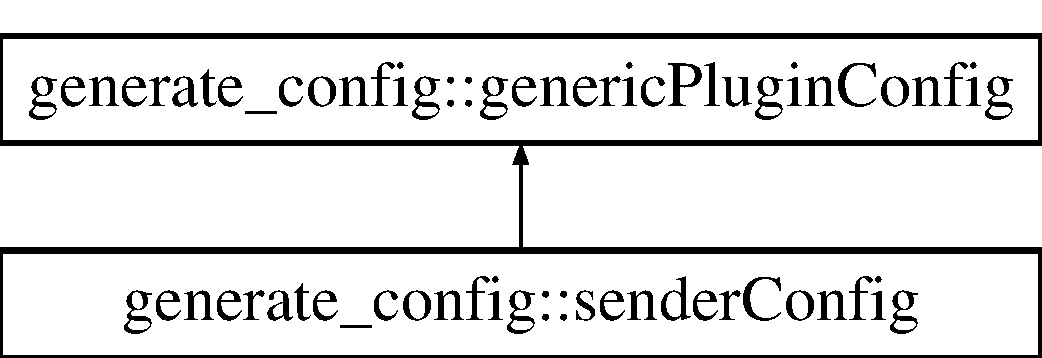
\includegraphics[height=2cm]{classgenerate__config_1_1senderConfig}
\end{center}
\end{figure}
\subsection*{Public Member Functions}
\begin{CompactItemize}
\item 
\hypertarget{classgenerate__config_1_1senderConfig_0eaa1e44dfc6199842d784e2211a6f67}{
def \textbf{\_\-\_\-init\_\-\_\-}}
\label{classgenerate__config_1_1senderConfig_0eaa1e44dfc6199842d784e2211a6f67}

\end{CompactItemize}


\subsection{Detailed Description}
Ask the user for specific config for the xPL sender. 

The documentation for this class was generated from the following file:\begin{CompactItemize}
\item 
config/generate\_\-config.py\end{CompactItemize}

\hypertarget{classgenerate__config_1_1triggerConfig}{
\section{generate\_\-config::triggerConfig Class Reference}
\label{classgenerate__config_1_1triggerConfig}\index{generate\_\-config::triggerConfig@{generate\_\-config::triggerConfig}}
}
Inheritance diagram for generate\_\-config::triggerConfig::\begin{figure}[H]
\begin{center}
\leavevmode
\includegraphics[height=2cm]{classgenerate__config_1_1triggerConfig}
\end{center}
\end{figure}
\subsection*{Public Member Functions}
\begin{CompactItemize}
\item 
\hypertarget{classgenerate__config_1_1triggerConfig_40e2f872feeb29963472a73ca7937dfd}{
def \textbf{\_\-\_\-init\_\-\_\-}}
\label{classgenerate__config_1_1triggerConfig_40e2f872feeb29963472a73ca7937dfd}

\end{CompactItemize}


\subsection{Detailed Description}


\footnotesize\begin{verbatim}
Ask the user for specific config for the xPL sender
\end{verbatim}
\normalsize
 

The documentation for this class was generated from the following file:\begin{CompactItemize}
\item 
config/generate\_\-config.py\end{CompactItemize}

\hypertarget{classx10API_1_1X10API}{
\section{x10API::X10API Class Reference}
\label{classx10API_1_1X10API}\index{x10API::X10API@{x10API::X10API}}
}
This class define some facilities to use X10.  


\subsection*{Public Member Functions}
\begin{CompactItemize}
\item 
\hypertarget{classx10API_1_1X10API_df1708474fd2eda336c665c64067a648}{
def \textbf{\_\-\_\-init\_\-\_\-}}
\label{classx10API_1_1X10API_df1708474fd2eda336c665c64067a648}

\item 
def \hyperlink{classx10API_1_1X10API_b23095bb54aa45e75857beaa59a7deed}{on}
\begin{CompactList}\small\item\em Send an ON order to the item element. \item\end{CompactList}\item 
def \hyperlink{classx10API_1_1X10API_37be53c20aaa39f5770a5085b80984bc}{off}
\begin{CompactList}\small\item\em Send an OFF order to the item element. \item\end{CompactList}\item 
def \hyperlink{classx10API_1_1X10API_d1e63a9dd573eb16a7d1009c72fac15e}{house\_\-on}
\begin{CompactList}\small\item\em Send an ALLON order to the item element. \item\end{CompactList}\item 
def \hyperlink{classx10API_1_1X10API_b04c7647aa5d80c462f0df36afaff4ec}{house\_\-off}
\begin{CompactList}\small\item\em Send an ALLOFF order to the item element. \item\end{CompactList}\end{CompactItemize}
\subsection*{Private Member Functions}
\begin{CompactItemize}
\item 
\hypertarget{classx10API_1_1X10API_398d98e0674a6cefaef1154eafe94a15}{
def \hyperlink{classx10API_1_1X10API_398d98e0674a6cefaef1154eafe94a15}{\_\-valid\_\-item}}
\label{classx10API_1_1X10API_398d98e0674a6cefaef1154eafe94a15}

\begin{CompactList}\small\item\em Check an item to have good 'HU' syntax Raise exception if it is not. \item\end{CompactList}\item 
\hypertarget{classx10API_1_1X10API_e9639dcec52e0f507fcc224a6c377c7d}{
def \hyperlink{classx10API_1_1X10API_e9639dcec52e0f507fcc224a6c377c7d}{\_\-valid\_\-house}}
\label{classx10API_1_1X10API_e9639dcec52e0f507fcc224a6c377c7d}

\begin{CompactList}\small\item\em Check an house to have good 'H' syntax Raise exception if it is not. \item\end{CompactList}\item 
def \hyperlink{classx10API_1_1X10API_268f590bc14835490b1ea823c86e4dcb}{\_\-send}
\begin{CompactList}\small\item\em Send a command trought heyu. \item\end{CompactList}\end{CompactItemize}
\subsection*{Private Attributes}
\begin{CompactItemize}
\item 
\hypertarget{classx10API_1_1X10API_e2bc653247758e1a67d8b8ac5b0d3611}{
\textbf{\_\-housecodes}}
\label{classx10API_1_1X10API_e2bc653247758e1a67d8b8ac5b0d3611}

\item 
\hypertarget{classx10API_1_1X10API_d2d5e02d43d6d4d1b0eba44248d29bb5}{
\textbf{\_\-unitcodes}}
\label{classx10API_1_1X10API_d2d5e02d43d6d4d1b0eba44248d29bb5}

\item 
\hypertarget{classx10API_1_1X10API_e11abda6663c0ad8d5e63d6abd52d562}{
\textbf{\_\-heyuconf}}
\label{classx10API_1_1X10API_e11abda6663c0ad8d5e63d6abd52d562}

\end{CompactItemize}


\subsection{Detailed Description}
This class define some facilities to use X10. 

It's based on heyu software, you need to have it installed and heyu binaries must be in your PATH 

\subsection{Member Function Documentation}
\hypertarget{classx10API_1_1X10API_268f590bc14835490b1ea823c86e4dcb}{
\index{x10API::X10API@{x10API::X10API}!\_\-send@{\_\-send}}
\index{\_\-send@{\_\-send}!x10API::X10API@{x10API::X10API}}
\subsubsection[\_\-send]{\setlength{\rightskip}{0pt plus 5cm}def x10API::X10API::\_\-send ( {\em self}, \/   {\em cmd}, \/   {\em item})\hspace{0.3cm}{\tt  \mbox{[}private\mbox{]}}}}
\label{classx10API_1_1X10API_268f590bc14835490b1ea823c86e4dcb}


Send a command trought heyu. 

\begin{Desc}
\item[Parameters:]
\begin{description}
\item[{\em cmd}]: Command to send ('ON','OFF', etc) \item[{\em item}]: Item to send order to (Can be HU or H form) \end{description}
\end{Desc}
\hypertarget{classx10API_1_1X10API_b23095bb54aa45e75857beaa59a7deed}{
\index{x10API::X10API@{x10API::X10API}!on@{on}}
\index{on@{on}!x10API::X10API@{x10API::X10API}}
\subsubsection[on]{\setlength{\rightskip}{0pt plus 5cm}def x10API::X10API::on ( {\em self}, \/   {\em item})}}
\label{classx10API_1_1X10API_b23095bb54aa45e75857beaa59a7deed}


Send an ON order to the item element. 

\begin{Desc}
\item[Parameters:]
\begin{description}
\item[{\em item}]: the item to send the ON order to  True if order was sent, False in case of errors \end{description}
\end{Desc}
\hypertarget{classx10API_1_1X10API_37be53c20aaa39f5770a5085b80984bc}{
\index{x10API::X10API@{x10API::X10API}!off@{off}}
\index{off@{off}!x10API::X10API@{x10API::X10API}}
\subsubsection[off]{\setlength{\rightskip}{0pt plus 5cm}def x10API::X10API::off ( {\em self}, \/   {\em item})}}
\label{classx10API_1_1X10API_37be53c20aaa39f5770a5085b80984bc}


Send an OFF order to the item element. 

\begin{Desc}
\item[Parameters:]
\begin{description}
\item[{\em item}]: the item to send the OFF order to  True if order was sent, False in case of errors \end{description}
\end{Desc}
\hypertarget{classx10API_1_1X10API_d1e63a9dd573eb16a7d1009c72fac15e}{
\index{x10API::X10API@{x10API::X10API}!house\_\-on@{house\_\-on}}
\index{house\_\-on@{house\_\-on}!x10API::X10API@{x10API::X10API}}
\subsubsection[house\_\-on]{\setlength{\rightskip}{0pt plus 5cm}def x10API::X10API::house\_\-on ( {\em self}, \/   {\em house})}}
\label{classx10API_1_1X10API_d1e63a9dd573eb16a7d1009c72fac15e}


Send an ALLON order to the item element. 

\begin{Desc}
\item[Parameters:]
\begin{description}
\item[{\em item}]: the item to send the ALLON order to  True if order was sent, False in case of errors \end{description}
\end{Desc}
\hypertarget{classx10API_1_1X10API_b04c7647aa5d80c462f0df36afaff4ec}{
\index{x10API::X10API@{x10API::X10API}!house\_\-off@{house\_\-off}}
\index{house\_\-off@{house\_\-off}!x10API::X10API@{x10API::X10API}}
\subsubsection[house\_\-off]{\setlength{\rightskip}{0pt plus 5cm}def x10API::X10API::house\_\-off ( {\em self}, \/   {\em house})}}
\label{classx10API_1_1X10API_b04c7647aa5d80c462f0df36afaff4ec}


Send an ALLOFF order to the item element. 

\begin{Desc}
\item[Parameters:]
\begin{description}
\item[{\em item}]: the item to send the ALLOFF order to  True if order was sent, False in case of errors \end{description}
\end{Desc}


The documentation for this class was generated from the following file:\begin{CompactItemize}
\item 
xpl/x10API.py\end{CompactItemize}

\hypertarget{classgenerate__config_1_1x10Config}{
\section{generate\_\-config::x10Config Class Reference}
\label{classgenerate__config_1_1x10Config}\index{generate\_\-config::x10Config@{generate\_\-config::x10Config}}
}
Inheritance diagram for generate\_\-config::x10Config::\begin{figure}[H]
\begin{center}
\leavevmode
\includegraphics[height=2cm]{classgenerate__config_1_1x10Config}
\end{center}
\end{figure}
\subsection*{Public Member Functions}
\begin{CompactItemize}
\item 
\hypertarget{classgenerate__config_1_1x10Config_ebb61db62b6f7df09e9061255514bb70}{
def \textbf{\_\-\_\-init\_\-\_\-}}
\label{classgenerate__config_1_1x10Config_ebb61db62b6f7df09e9061255514bb70}

\end{CompactItemize}


\subsection{Detailed Description}


\footnotesize\begin{verbatim}
Ask the user for specific config for X10 xPL module
\end{verbatim}
\normalsize
 

The documentation for this class was generated from the following file:\begin{CompactItemize}
\item 
config/generate\_\-config.py\end{CompactItemize}

\hypertarget{classx10API_1_1X10Exception}{
\section{x10API::X10Exception Class Reference}
\label{classx10API_1_1X10Exception}\index{x10API::X10Exception@{x10API::X10Exception}}
}
X10 exception.  


\subsection*{Public Member Functions}
\begin{CompactItemize}
\item 
\hypertarget{classx10API_1_1X10Exception_033a895f90bdb03c500be02471701831}{
def \textbf{\_\-\_\-init\_\-\_\-}}
\label{classx10API_1_1X10Exception_033a895f90bdb03c500be02471701831}

\item 
\hypertarget{classx10API_1_1X10Exception_a9a0adf2ba11276fecd3d7d0f759a8c9}{
def \textbf{\_\-\_\-str\_\-\_\-}}
\label{classx10API_1_1X10Exception_a9a0adf2ba11276fecd3d7d0f759a8c9}

\end{CompactItemize}
\subsection*{Public Attributes}
\begin{CompactItemize}
\item 
\hypertarget{classx10API_1_1X10Exception_ea0d93a4bd33db7e6f416fe28d739c84}{
\textbf{value}}
\label{classx10API_1_1X10Exception_ea0d93a4bd33db7e6f416fe28d739c84}

\end{CompactItemize}


\subsection{Detailed Description}
X10 exception. 

The documentation for this class was generated from the following file:\begin{CompactItemize}
\item 
xpl/x10API.py\end{CompactItemize}

\hypertarget{classdatetime_1_1xPLDateTime}{
\section{datetime::xPLDateTime Class Reference}
\label{classdatetime_1_1xPLDateTime}\index{datetime::xPLDateTime@{datetime::xPLDateTime}}
}
\subsection*{Public Member Functions}
\begin{CompactItemize}
\item 
\hypertarget{classdatetime_1_1xPLDateTime_b39a3cb860ddd3595e348bc7f910f1e4}{
def \textbf{\_\-\_\-init\_\-\_\-}}
\label{classdatetime_1_1xPLDateTime_b39a3cb860ddd3595e348bc7f910f1e4}

\end{CompactItemize}
\subsection*{Private Member Functions}
\begin{CompactItemize}
\item 
def \hyperlink{classdatetime_1_1xPLDateTime_56f581af02f2f66b6b8d21fe910b9b5d}{\_\-f}
\item 
def \hyperlink{classdatetime_1_1xPLDateTime_8705cd0ed46a76dda2d82c1a87fc1b3e}{\_\-send\_\-datetime}
\end{CompactItemize}
\subsection*{Private Attributes}
\begin{CompactItemize}
\item 
\hypertarget{classdatetime_1_1xPLDateTime_1b15c71df12789d777f44dc8d39e48f9}{
\textbf{\_\-\_\-myxpl}}
\label{classdatetime_1_1xPLDateTime_1b15c71df12789d777f44dc8d39e48f9}

\item 
\hypertarget{classdatetime_1_1xPLDateTime_7d66e43fe5cd70d3e9c8a90ae406dcc7}{
\textbf{\_\-timer}}
\label{classdatetime_1_1xPLDateTime_7d66e43fe5cd70d3e9c8a90ae406dcc7}

\end{CompactItemize}


\subsection{Detailed Description}


\footnotesize\begin{verbatim}
Send date and time on the xPL network every minute
\end{verbatim}
\normalsize
 

\subsection{Member Function Documentation}
\hypertarget{classdatetime_1_1xPLDateTime_56f581af02f2f66b6b8d21fe910b9b5d}{
\index{datetime::xPLDateTime@{datetime::xPLDateTime}!\_\-f@{\_\-f}}
\index{\_\-f@{\_\-f}!datetime::xPLDateTime@{datetime::xPLDateTime}}
\subsubsection[\_\-f]{\setlength{\rightskip}{0pt plus 5cm}def datetime::xPLDateTime::\_\-f ( {\em self}, \/   {\em nb})\hspace{0.3cm}{\tt  \mbox{[}private\mbox{]}}}}
\label{classdatetime_1_1xPLDateTime_56f581af02f2f66b6b8d21fe910b9b5d}




\footnotesize\begin{verbatim}
Format the number
\end{verbatim}
\normalsize
 \hypertarget{classdatetime_1_1xPLDateTime_8705cd0ed46a76dda2d82c1a87fc1b3e}{
\index{datetime::xPLDateTime@{datetime::xPLDateTime}!\_\-send\_\-datetime@{\_\-send\_\-datetime}}
\index{\_\-send\_\-datetime@{\_\-send\_\-datetime}!datetime::xPLDateTime@{datetime::xPLDateTime}}
\subsubsection[\_\-send\_\-datetime]{\setlength{\rightskip}{0pt plus 5cm}def datetime::xPLDateTime::\_\-send\_\-datetime ( {\em self})\hspace{0.3cm}{\tt  \mbox{[}private\mbox{]}}}}
\label{classdatetime_1_1xPLDateTime_8705cd0ed46a76dda2d82c1a87fc1b3e}




\footnotesize\begin{verbatim}
Send date and time on xPL network
\end{verbatim}
\normalsize
 

The documentation for this class was generated from the following file:\begin{CompactItemize}
\item 
xpl/datetime.py\end{CompactItemize}

\hypertarget{classxPLAPI_1_1XPLException}{
\section{xPLAPI::XPLException Class Reference}
\label{classxPLAPI_1_1XPLException}\index{xPLAPI::XPLException@{xPLAPI::XPLException}}
}
xPL exception  


\subsection*{Public Member Functions}
\begin{CompactItemize}
\item 
\hypertarget{classxPLAPI_1_1XPLException_fa97cb40136ea6f52c5b9ce792435e75}{
def \textbf{\_\-\_\-init\_\-\_\-}}
\label{classxPLAPI_1_1XPLException_fa97cb40136ea6f52c5b9ce792435e75}

\item 
\hypertarget{classxPLAPI_1_1XPLException_2713888a5319bbbeb96a991547dd127b}{
def \textbf{\_\-\_\-str\_\-\_\-}}
\label{classxPLAPI_1_1XPLException_2713888a5319bbbeb96a991547dd127b}

\end{CompactItemize}
\subsection*{Public Attributes}
\begin{CompactItemize}
\item 
\hypertarget{classxPLAPI_1_1XPLException_a426e1d994b5f51ef4249260b8357de7}{
\textbf{value}}
\label{classxPLAPI_1_1XPLException_a426e1d994b5f51ef4249260b8357de7}

\end{CompactItemize}


\subsection{Detailed Description}
xPL exception 

The documentation for this class was generated from the following file:\begin{CompactItemize}
\item 
xpl/xPLAPI.py\end{CompactItemize}

\hypertarget{classxPLAPI_1_1xPLTimer}{
\section{xPLAPI::xPLTimer Class Reference}
\label{classxPLAPI_1_1xPLTimer}\index{xPLAPI::xPLTimer@{xPLAPI::xPLTimer}}
}
\subsection*{Public Member Functions}
\begin{CompactItemize}
\item 
def \hyperlink{classxPLAPI_1_1xPLTimer_e651d6889d77aabd9227e622d5821d14}{\_\-\_\-init\_\-\_\-}
\item 
def \hyperlink{classxPLAPI_1_1xPLTimer_f9e579ecf5a8e2b2ed86ce78c5029a0e}{start}
\item 
def \hyperlink{classxPLAPI_1_1xPLTimer_2a04504c8d29908bc6601879fe63aa23}{stop}
\end{CompactItemize}
\subsection*{Private Member Functions}
\begin{CompactItemize}
\item 
def \hyperlink{classxPLAPI_1_1xPLTimer_59ac53c691fadf44bf28fb74a226251f}{\_\-run}
\end{CompactItemize}
\subsection*{Private Attributes}
\begin{CompactItemize}
\item 
\hypertarget{classxPLAPI_1_1xPLTimer_cf45a98a98a98ce25ae50665771d1e92}{
\textbf{\_\-callback}}
\label{classxPLAPI_1_1xPLTimer_cf45a98a98a98ce25ae50665771d1e92}

\item 
\hypertarget{classxPLAPI_1_1xPLTimer_a5189f41b3d558ccef9411af7c563796}{
\textbf{\_\-time}}
\label{classxPLAPI_1_1xPLTimer_a5189f41b3d558ccef9411af7c563796}

\item 
\hypertarget{classxPLAPI_1_1xPLTimer_f2a85e94f12015c68fb34b4461476cc3}{
\textbf{\_\-timer}}
\label{classxPLAPI_1_1xPLTimer_f2a85e94f12015c68fb34b4461476cc3}

\end{CompactItemize}


\subsection{Detailed Description}


\footnotesize\begin{verbatim}
xPLTimer will call a callback function each n seconds
\end{verbatim}
\normalsize
 

\subsection{Member Function Documentation}
\hypertarget{classxPLAPI_1_1xPLTimer_e651d6889d77aabd9227e622d5821d14}{
\index{xPLAPI::xPLTimer@{xPLAPI::xPLTimer}!\_\-\_\-init\_\-\_\-@{\_\-\_\-init\_\-\_\-}}
\index{\_\-\_\-init\_\-\_\-@{\_\-\_\-init\_\-\_\-}!xPLAPI::xPLTimer@{xPLAPI::xPLTimer}}
\subsubsection[\_\-\_\-init\_\-\_\-]{\setlength{\rightskip}{0pt plus 5cm}def xPLAPI::xPLTimer::\_\-\_\-init\_\-\_\- ( {\em self}, \/   {\em time}, \/   {\em cb})}}
\label{classxPLAPI_1_1xPLTimer_e651d6889d77aabd9227e622d5821d14}




\footnotesize\begin{verbatim}
Constructor : create the internal timer
@param time : time of loop in second
@param cb : callback function which will be call eact 'time' seconds
\end{verbatim}
\normalsize
 \hypertarget{classxPLAPI_1_1xPLTimer_59ac53c691fadf44bf28fb74a226251f}{
\index{xPLAPI::xPLTimer@{xPLAPI::xPLTimer}!\_\-run@{\_\-run}}
\index{\_\-run@{\_\-run}!xPLAPI::xPLTimer@{xPLAPI::xPLTimer}}
\subsubsection[\_\-run]{\setlength{\rightskip}{0pt plus 5cm}def xPLAPI::xPLTimer::\_\-run ( {\em self})\hspace{0.3cm}{\tt  \mbox{[}private\mbox{]}}}}
\label{classxPLAPI_1_1xPLTimer_59ac53c691fadf44bf28fb74a226251f}




\footnotesize\begin{verbatim}
internal timer loopback function
\end{verbatim}
\normalsize
 \hypertarget{classxPLAPI_1_1xPLTimer_f9e579ecf5a8e2b2ed86ce78c5029a0e}{
\index{xPLAPI::xPLTimer@{xPLAPI::xPLTimer}!start@{start}}
\index{start@{start}!xPLAPI::xPLTimer@{xPLAPI::xPLTimer}}
\subsubsection[start]{\setlength{\rightskip}{0pt plus 5cm}def xPLAPI::xPLTimer::start ( {\em self})}}
\label{classxPLAPI_1_1xPLTimer_f9e579ecf5a8e2b2ed86ce78c5029a0e}




\footnotesize\begin{verbatim}
Start the timer
\end{verbatim}
\normalsize
 \hypertarget{classxPLAPI_1_1xPLTimer_2a04504c8d29908bc6601879fe63aa23}{
\index{xPLAPI::xPLTimer@{xPLAPI::xPLTimer}!stop@{stop}}
\index{stop@{stop}!xPLAPI::xPLTimer@{xPLAPI::xPLTimer}}
\subsubsection[stop]{\setlength{\rightskip}{0pt plus 5cm}def xPLAPI::xPLTimer::stop ( {\em self})}}
\label{classxPLAPI_1_1xPLTimer_2a04504c8d29908bc6601879fe63aa23}




\footnotesize\begin{verbatim}
Stop the timer
\end{verbatim}
\normalsize
 

The documentation for this class was generated from the following file:\begin{CompactItemize}
\item 
xpl/xPLAPI.py\end{CompactItemize}

\printindex
\end{document}
